\documentclass[letterpaper,12pt]{article}
\usepackage[utf8]{inputenc}
\usepackage{fullpage}
\usepackage{courier}
\usepackage[margin=0.75in]{geometry}
\usepackage{listings}
\usepackage{color}
\usepackage{graphicx}
\usepackage[width=4in]{caption}
\usepackage{hyphenat}

% define extra colors
\definecolor{dkgreen}{rgb}{0,0.6,0}
\definecolor{purple}{RGB}{159,0,197}

\newcommand*\unparagraph{%
	\par
	\nopagebreak
	\vskip3.25ex plus1ex minus.2ex
	\noindent
}

\lstset{
	language=C++,
	basicstyle=\ttfamily,
	backgroundcolor=\color{white},
	showspaces=false,
	showstringspaces=false,
	frame=single,
	tabsize=3,
	keywordstyle=\color{purple},
	commentstyle=\color{dkgreen},
	stringstyle=\color{blue},
	escapeinside={\%*}{*)}
}

\title{\Large CS 1428\\Lab 4 Sections L06 and L19} 
\author{Jared Wallace}
\date{}

\begin{document}

\maketitle

\section*{Topic} Today we will be talking about relational operators and conditional statements.

Relational operators are the operators that allow us to form relational expressions. Conditional
statements are the control structures that we use to take advantage of relational expressions and
alter the flow of the program to our benefit.

\unparagraph{}
\begin{lstlisting}[basicstyle=\footnotesize\ttfamily]
/* A stand alone relational expression.  Note, this statement is pointless and 
   has no effect on the execution of the program whatsoever. */
intOne > intTwo;

/* The above statement might be of use if we stored the result into a variable 
   with the type bool.

   In most cases that would be a pointless complication.  The standard way to make 
   use of relational expressions is with the use of conditional statements. */
if (intOne > intTwo)
	cout << "The variable intOne is greater than intTwo!" << endl;

/* We can also make use of mutually exclusive possibilities by utilizing the else 
   and else if control structures. */
if (num > 0)
	cout << "The variable num is positive!" << endl;
else if (num < 0)
	cout << "The variable num is negative!" << endl;
else
	cout << "The variable num has the value 0 and"
	     << "therefore is neither positive or negative!" << endl;

/* When we desire to execute multiple lines in response to a conditional we must
   use the curly braces to group them. */
if (!fin)
{
	cout << "The file did not open as expected!" << endl;
	return 0;
}
\end{lstlisting}

\newpage

\section*{Questions}
\begin{enumerate}
	\item Which of the following is not a relational operator?
		\begin{enumerate}
			\item \lstinline$<=$
			\item \lstinline$=$
			\item \lstinline$>=$
			\item \lstinline$>$
		\end{enumerate}
	\item \nohyphens{Write a relational expression that checks for whether or not two integers (firstInt and secondInt) are \textbf{NOT} equal.}
		\vspace{20mm}
	\item You need to trace the execution of the following code and determine what the final value of $x$ is.
		\lstinputlisting[basicstyle=\footnotesize\ttfamily,frame=none,keywordstyle=\color{black},commentstyle=\color{black},stringstyle=\color{black}]{labsnippet.cpp}
		\begin{enumerate}
			\item 12
			\item 14
			\item 17
			\item 9
		\end{enumerate}

\end{enumerate}

\section*{Letter Grade Assignment Program}
Write a program that prompts the user for a grade.  The program will first
verify that the entered grade is valid (0 $\le$ grade $\le$ 100). \textbf{If the grade is invalid
then an error is printed} (use cerr instead of cout).  If the grade is valid then you should determine 
which letter grade corresponds to the number entered. Then you need to print a response like "The grade you entered is an A".

\vspace{5mm}

\begin{table}[h]
	\centering
	\begin{tabular}{|c|c|}
		90 - 100 & A \\
		80 - 89  & B \\
		70 - 79  & C \\
		0  - 69  & F \\
	\end{tabular}
\end{table}

\vspace{10mm}

\unparagraph{} \textbf{When you are done print out your source file, staple it to this
page and write your name at the top before turning it in. Do not forget to upload your
source file through the homework upload utility.}

\vspace{20mm}

\begin{figure}[ht!]
	\centering
	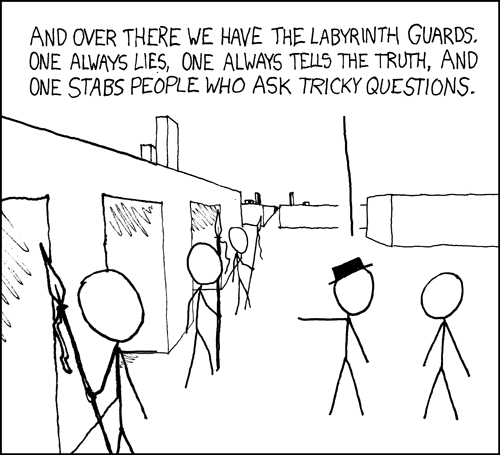
\includegraphics[width=4in]{labyrinth_puzzle.png}
	\caption*{And the whole setup is just a trap to capture 
	escaping logicians. None of the doors actually lead out.}
\end{figure}

\end{document}
